\documentclass[journal, a4paper]{IEEEtran}

\usepackage{graphicx}
\usepackage{caption}
\usepackage{subcaption}
% some very useful LaTeX packages include:

%\usepackage{cite}
\usepackage{graphicx}
\usepackage{amsmath,eqparbox,booktabs,xparse}
\usepackage{smartdiagram}
\usetikzlibrary{quotes}
%\usepackage{psfrag}   
%\usepackage{subfigure}
\usepackage{neuralnetwork}
\usepackage{url}        % Written by Donald Arseneau
%\usepackage{stfloats}  % Written by Sigitas Tolusis
\usepackage{xcolor}
%\interdisplaylinepenalty=2500
\usepackage{listings}

\lstset{basicstyle=\ttfamily, keywordstyle=\bfseries}
\usetikzlibrary{arrows.meta, positioning}
\tikzset{%
    block/.style = {draw=gray, rectangle, thick,
        minimum height=6em, text width=4em, align=center}
}

\makeatletter
\NewDocumentCommand{\eqmathbox}{o O{c} m}{%
  \IfValueTF{#1}
    {\def\eqmathbox@##1##2{\eqmakebox[#1][#2]{$##1##2$}}}
    {\def\eqmathbox@##1##2{\eqmakebox{$##1##2$}}}
  \mathpalette\eqmathbox@{#3}
}
% Your document starts here!
\begin{document}

% Define document title and author
	\title{Project 1 of Deep Learning\\ \textit{\Large{Classification, weight sharing, auxiliary losses}}}
	\author{Francis \textbf{Damachi} - Costanza \textbf{Volpini}}
	\markboth{Project 1 - Deep Learning EE559 - EPFL}{}
	\maketitle
	
\begin{abstract}
The aim of this project was to show the impact of weight sharing and the use of auxiliary loss. The task was to compare two digits in a two-channel image. Starting from linear model until some more complex non-linear model, we have found out that convolutional neural networks represents the best solution to classify images.
\end{abstract}

\section{Introduction}
\label{sec:intro}
\textit{Convolutional neural network} (CNN) represents the most powerful model to analyse images. Indeed, CNN uses the pixel locality to learn better. 

We have started the project training simple linear models, in particular \textit{Linear Regression} and \textit{Logistic Regression} (see Section \ref{sec:linearmodel}) but we have notice that these models are too simple and not consider the pixel locality. We have then used a more complex model \textit{Neural Network} with one-loss and two-losses (as explained and showed in Section \ref{sec:nnmodel}), we got a bad accuracy caused by the fact that we have a model composed by just linear layer. The last model that we have implemented is the \textit{Convolutional neural network}, with this model we got a very good approximation (see Section \ref{sec:cnnmodel}).
In all the models, we have used \textit{Adam's method} instead of \textit{stochastic gradient descent} as optimizer since it use an adaptive learning rate (the learning rate of SGD has an equivalent type of effect for all the weights/parameters of the model \cite{reference0}).
As criterion, we have used \textit{Mean Square Error} for all the models.


Section \ref{sec:data} explain the structure of the dataset, Section \ref{sec:codestruc} describes briefly the content of each file. In Section \ref{sec:comparison}, \ref{sec:conclusion} we have showed the performance accuracy obtained by each model with a fixed seed, explaining why we got these results.


\section{Data}
\label{sec:data}
The data set consists of an input series of $2\times14\times14$ tensor (2 images in grayscale). Training and test set is $1000$ pairs each. In total we will have six tensors: images ($N\times2\times14\times14$), prediction (boolean), classes of the two digits ($N\times2$), both for training and test sets. The MNIST database is composed by handwritten digits (from $0$ to $9$); to load the dataset we have used the provided function \texttt{generate\_pair\_sets(N)}.

\section{Code structure}
\label{sec:codestruc}
In this section contains the description of each file.
\begin{itemize}
    \item \texttt{scripts/data.py}: class to generate the dataset. Contains different methods (e.g. flat the input, get a dataset in 2D or in 3D, enable the hot-encoding).
    \item \texttt{scripts/model.py}: general class to define a model to train and test it (with corresponding plot and history).
    \item \texttt{scripts/models\_implemented.py}: contains all the model classes (e.g. NNModel1Loss, CNNModel2Loss).
    \item \texttt{main.py}: contains examples of each models, in order to call and train a model.
\end{itemize}

\section{Linear Models}
\label{sec:linearmodel}
We have implemented \textit{Linear Regression} and \textit{Logistic Regression}. Regression is represented by a final layer that it is linear. In the logistic regression we have used a sigmoid as an activation function in the output layer. A linear layer accept as input a vector of values, that is the reason why we need to flat the input (the raw input is composed by 2D images). In fact a linear layer give a weight to each pixel, then it will accept a vector composed by N rows and D dimensions (columns), in our case it will have size $14 \times 14 \times 2$.

% CNN sfrutta localita pixel e le tratta come img - no flatten.

% ASCOLTARE DA AUDIO 19 Aprile

%TODO: mettere size flatted come input???
\begin{figure}[!h]
    \centering
    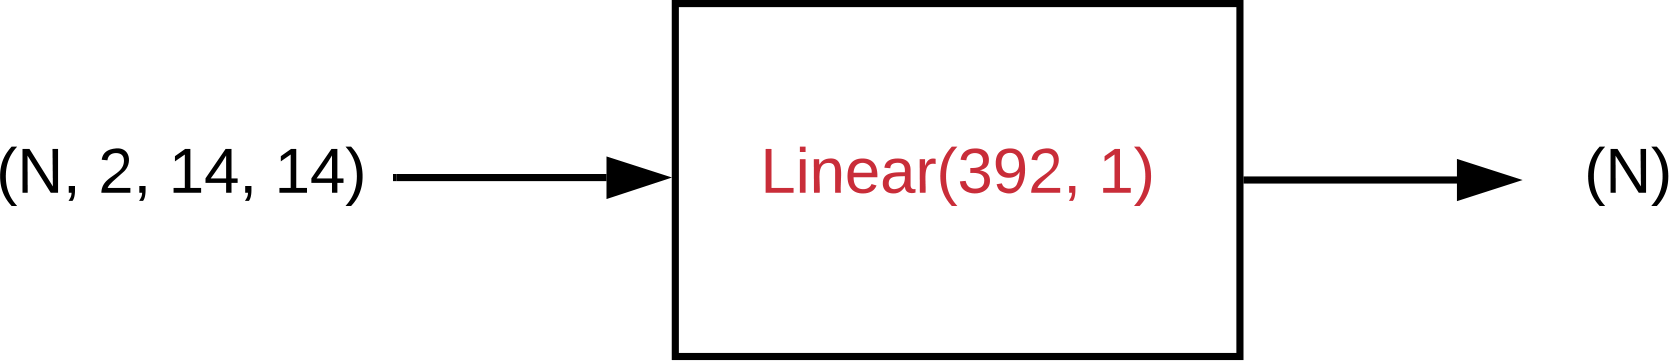
\includegraphics[width=0.4\textwidth]{linearregression.png}
    \caption{Linear Regression model}
    \label{fig:linearregression}
\end{figure}

\begin{figure}[!h]
    \centering
    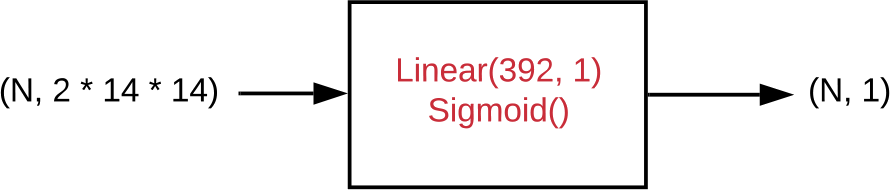
\includegraphics[width=0.4\textwidth]{logistic.png}
    \caption{Logistic Regression model}
    \label{fig:logisticregression}
\end{figure}

\section{Neural Network Models}
\label{sec:nnmodel}

\section{Convolutional Neural Network Models}
\label{sec:cnnmodel}

\section{Comparison of models}
\label{sec:comparison}

\section{Conclusion}
\label{sec:conclusion}
% %%%%%%%%%%%%%%%%%%%%%



% Now we need a bibliography:
\begin{thebibliography}{999}

	%Each item starts with a \bibitem{reference} command and the details thereafter.
	\bibitem{reference0}
    	optim.Adam vs optim.SGD. Let’s dive in.
    	\url{https://medium.com/@Biboswan98/optim-adam-vs-optim-sgd-lets-dive-in-8dbf1890fbdc}
	
% 	\bibitem{reference1}
% 	    Neural networks and deep learning, Michael Nielsen.
	    
%     \bibitem{reference2}
%     Notes of course Deep Learning (EE-559), Prof. François Fleuret.

\end{thebibliography}

% Your document ends here!
\end{document}